\documentclass[a4paper,11pt]{article}
\usepackage{amsmath}
\usepackage{amsthm}
\usepackage{amssymb}
\usepackage{graphicx}
%\usepackage{fancyhdr}
\usepackage{hyperref}

% Use Times fonts
%\usepackage{mathptmx}
\usepackage[scaled]{helvet}
\renewcommand{\ttdefault}{pcr}
\usepackage{bm}

\setlength{\oddsidemargin}{0pt}   %%% left margin
\setlength{\textwidth}{159.2mm}
\setlength{\topmargin}{0mm}
\setlength{\headheight}{10mm}
\setlength{\headsep}{10mm}         %%% length between header and test
\setlength{\textheight}{219.2mm}

\setlength{\parindent}{0pt}

%%
\newtheorem{formula}{Formula}[section]

%\pagestyle{fancy}
%\renewcommand{\headrulewidth}{0pt}
%\fancyhf{}
%\rhead{JK 0000 - \thepage}
%\rfoot{\url{http://www.github.com/junkoda/mock_zeldovich}}

\begin{document}

\section{Linear approximation to the Zel'dovich mock}

\subsection{Configuration}

We consider particles perturbed from a lattice at,
\begin{equation}
  \bm{q}^{i,j,k} = (i, j, k) \Delta x,
\end{equation}
where $i, j, k$ are integers, with the Zel'dovich displacements,
\begin{equation}
  \bm{x}^{i,j,k} = \bm{q}^{i,j,k} + \bm{\Psi}^{i,j,k},
\end{equation}
and the density field computed on grid points
shifted by half particle separation using CIC mass assignment,
\begin{equation}
  \bm{x}_\mathrm{grid}^{i,j,k} =
    \left(i + \frac{1}{2}, j + \frac{1}{2}, k+\frac{1}{2} \right) \Delta x.
\end{equation}

The number of grid points are equal to the number of particles. This
is the simplest case and other configuration can be calculated in a
similar way.


\subsection{Analytical solution to discrete Zel'dovich}

The number density at a grid point $\bm{x}^\mathrm{grid}$ is,
\begin{equation}
  n(\bm{x}^\mathrm{grid}) =
  \sum_{i', j', k'} W(x^\mathrm{grid}_1 - x_1^{i', j', k'})
                  W(x^\mathrm{grid}_2 - x_2^{i', j', k'})
                  W(x^\mathrm{grid}_3 - x_3^{i', j', k'})
\end{equation}

where the mass assignment kernel $W$ for CIC is,
\begin{equation}
  W(x) = 
  \begin{cases}
  
    1 - |x|/\Delta x &\text{if } |x| < \Delta x,\\
    0                & \text{otherwise}.
  \end{cases}
\end{equation}
The unit of $n$ is number of particles per cell;
mean density is 1.

The density at grid point $(i, j, k)$ has contribution from 8 neighbour particles,
\begin{equation}
  \label{eq:n-nonlinear}
\begin{split}
  n_{i,j,k} &= \left( \frac{1}{2} - \Psi_1^{i,   j,   k  }/\Delta x \right)
              \left( \frac{1}{2} - \Psi_2^{i,   j,   k  }/\Delta x \right)
              \left( \frac{1}{2} - \Psi_3^{i,   j,   k  }/\Delta x \right)\\
           &+ \left( \frac{1}{2} + \Psi_1^{i+1, j,   k  }/\Delta x \right)
              \left( \frac{1}{2} - \Psi_2^{i+1, j,   k  }/\Delta x \right)
              \left( \frac{1}{2} - \Psi_3^{i+1, j,   k  }/\Delta x \right)\\
           &+ \left( \frac{1}{2} - \Psi_1^{i,   j+1, k  }/\Delta x \right)
              \left( \frac{1}{2} + \Psi_2^{i,   j+1, k  }/\Delta x \right)
              \left( \frac{1}{2} - \Psi_3^{i,   j+1, k  }/\Delta x \right)\\
           &+ \left( \frac{1}{2} + \Psi_1^{i+1, j+1, k  }/\Delta x \right)
              \left( \frac{1}{2} + \Psi_2^{i+1, j+1, k  }/\Delta x \right)
              \left( \frac{1}{2} - \Psi_3^{i+1, j+1, k  }/\Delta x \right)\\
           &+ \left( \frac{1}{2} - \Psi_1^{i,   j  , k+1}/\Delta x \right)
              \left( \frac{1}{2} - \Psi_2^{i,   j  , k+1}/\Delta x \right)
              \left( \frac{1}{2} + \Psi_3^{i,   j  , k+1}/\Delta x \right)\\
           &+ \left( \frac{1}{2} + \Psi_1^{i+1, j  , k+1}/\Delta x \right)
              \left( \frac{1}{2} - \Psi_2^{i+1, j  , k+1}/\Delta x \right)
              \left( \frac{1}{2} + \Psi_3^{i+1, j  , k+1}/\Delta x \right)\\
           &+ \left( \frac{1}{2} - \Psi_1^{i,   j+1, k+1}/\Delta x \right)
              \left( \frac{1}{2} + \Psi_2^{i,   j+1, k+1}/\Delta x \right)
              \left( \frac{1}{2} + \Psi_3^{i,   j+1, k+1}/\Delta x \right)\\
           &+ \left( \frac{1}{2} + \Psi_1^{i+1, j+1, k+1}/\Delta x \right)
              \left( \frac{1}{2} + \Psi_2^{i+1, j+1, k+1}/\Delta x \right)
              \left( \frac{1}{2} + \Psi_3^{i+1, j+1, k+1}/\Delta x \right),
\end{split}
\end{equation}
given that all displacements are smaller than half grid spacing
$|\Psi_i| \le \frac{1}{2} \Delta x$.

The linear approximation for small $\Psi$ is,
\begin{equation}
  \label{eq:n-linear}
\begin{split}
  n_{i,j,k} = 1 + \frac{1}{4 \Delta x} \Big[
   & - \Psi_1^{i,   j,   k  } - \Psi_2^{i,   j,   k  } - \Psi_3^{i,   j,   k  }\\
   & + \Psi_1^{i+1, j,   k  } - \Psi_2^{i+1, j,   k  } - \Psi_3^{i+1, j,   k  }\\
   & - \Psi_1^{i,   j+1, k  } + \Psi_2^{i,   j+1, k  } - \Psi_3^{i,   j+1, k  }\\
   & + \Psi_1^{i+1, j+1, k  } + \Psi_2^{i+1, j+1, k  } - \Psi_3^{i+1, j+1, k  }\\
   & - \Psi_1^{i,   j  , k+1} - \Psi_2^{i,   j  , k+1} + \Psi_3^{i,   j  , k+1}\\
   & + \Psi_1^{i+1, j  , k+1} - \Psi_2^{i+1, j  , k+1} + \Psi_3^{i+1, j  , k+1}\\
   & - \Psi_1^{i,   j+1, k+1} + \Psi_2^{i,   j+1, k+1} + \Psi_3^{i,   j+1, k+1}\\
   & + \Psi_1^{i+1, j+1, k+1} + \Psi_2^{i+1, j+1, k+1} + \Psi_3^{i+1, j+1, k+1}
   \Big]
\end{split}
\end{equation}

In Fourier space, the translation becomes an exponential factor, e.g., 
\begin{equation}
  \hat{\Psi}_1^{i+1, j, k} = e^{i k_1 \Delta x} \hat{\Psi}_1^{i,j,k},
\end{equation}
where, $\hat{\Psi}^{i,j,k}$ is the Fourier transform of $\Psi^{i, j, k}$
at wavenumber $\bm{k} = \frac{2\pi}{L} (i, j, k)$.

The terms proportional to $\Psi_1$ becomes
\begin{equation}
\begin{split}
  &-\frac{1}{4\Delta x} \left[
    (1 - e^{i k_x \Delta x}) + (1 - e^{i k_x \Delta x}) e^{i k_y \Delta x}
    + (1 - e^{i k_x \Delta x}) e^{i k_z \Delta x}
    + (1 - e^{i k_x \Delta x}) e^{i k_y \Delta x} e^{i k_z \Delta x} \right]
  \hat{\Psi}_1^{i, j, k}\\
  &= -\frac{1}{4 \Delta x}
       (1 - e^{i k_x \Delta x})(1 + e^{i k_y \Delta x} + e^{i k_z \Delta x} +
         e^{i k_y \Delta x} e^{i k_z \Delta x}) \hat{\Psi}_1^{i,j,k}\\
  &= -\frac{1}{4 \Delta x}
         (1 - e^{i k_x \Delta x})(1 + e^{i k_y \Delta x})(1 +  e^{i k_z \Delta x})
         \hat{\Psi}_1^{i,j,k}\\
  &= -\frac{2}{\Delta x} e^{\frac{i}{2} (k_x + k_y + k_z) \Delta x} 
         \sin \left( \frac{1}{2} k_x \Delta x \right)
         \cos \left( \frac{1}{2} k_y \Delta x \right)
         \cos \left(\frac{1}{2} k_z \Delta x \right)
         \hat{\Psi}_1^{i,j,k}
\end{split}
\end{equation}

We express the density contrast $\delta = n - 1$ in terms of
the input density contrast $\delta_\mathrm{in}$. The Zel'dovich
displacement in Fourier space is,
\begin{equation}
  \hat{\bm{\Psi}}(\bm{k}) = -\frac{i\bm{k}}{k^2} \hat{\delta}_\mathrm{in}(\bm{k}).
\end{equation}

The calculation so far gives the window function for the density
field on a grid for particles on lattice perturbed by the Zel'dovich
approximation in the linear limit:

\begin{equation}
  \hat{\delta}(\bm{k}) = e^{\frac{i}{2}  (k_x + k_y + k_z) \Delta x} W_\mathrm{Zel}(\bm{k}) \hat{\delta}_\mathrm{in}(\bm{k}),
\end{equation}

\begin{equation}
\begin{split}
  W_\mathrm{Zel}(\bm{k}) = \frac{2}{k^2 \Delta x}
              \bigg[
      &k_x \sin\left( \frac{1}{2} k_x \Delta x \right)
        \cos\left( \frac{1}{2} k_y \Delta x \right)
        \cos\left( \frac{1}{2} k_z \Delta x \right)\\
    + &k_y \cos\left( \frac{1}{2} k_x \Delta x \right)
        \sin\left( \frac{1}{2} k_y \Delta x \right)
        \cos\left( \frac{1}{2} k_z \Delta x \right)\\
    + &k_z \cos\left( \frac{1}{2} k_x \Delta x \right)
        \cos\left( \frac{1}{2} k_y \Delta x \right)
        \sin\left( \frac{1}{2} k_z \Delta x \right) \bigg]
    \hat{\delta}_\mathrm{in}(\bm{k}).
\end{split}
\end{equation}

The power spectrum
\begin{equation}
  \label{eq:power-spectrum}
  P_\mathrm{Zel}(\bm{k}) =  |W_\mathrm{Zel}(\bm{k})|^2 P_\mathrm{in}(k)
\end{equation}

In essence, the window function for $P_\mathrm{Zel}$ is different from
the usual window function for CIC mass assignment due to the specific displacement
between the initial lattice and the grid points.


\section{Numerical result}

Box size $L = 375 \, h^{-1} \mathrm{Mpc}$, $256^3$ grid points, scale
factor is $a=0.01$.

\begin{figure}
  \centering
  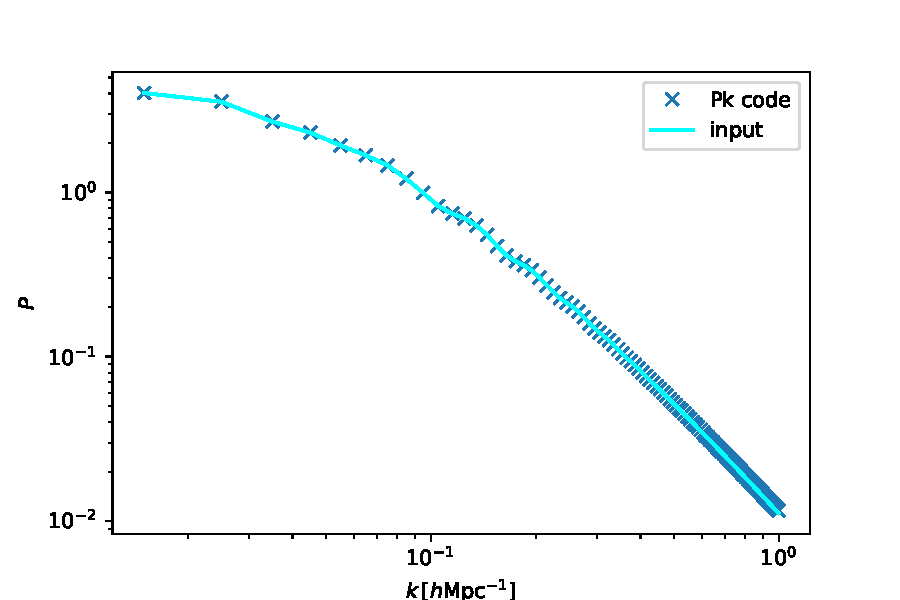
\includegraphics{zeldovich_linear1.pdf}
  \caption{Zel'dovich power spectrum at scale factor $a=0.01$}
\end{figure}

\begin{figure}
  \centering
  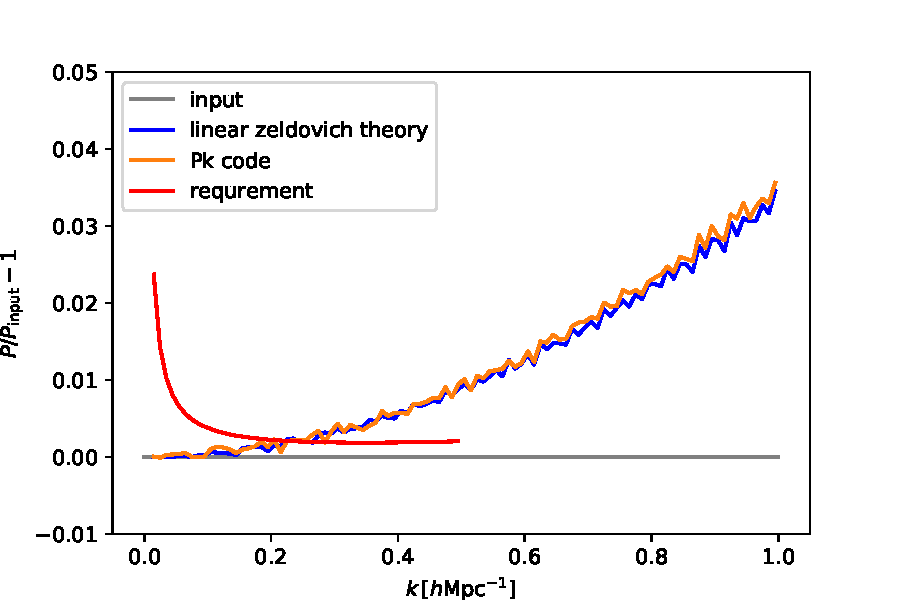
\includegraphics{zeldovich_linear2.pdf}
  \caption{Relative difference between the Zel'dovich power spectrum
    and the input power spectrum. The linear Zel'dovich theory is
    equation~(\ref{eq:power-spectrum}) with CIC mass assignment
    correction.}
\end{figure}

\begin{figure}
  \centering
  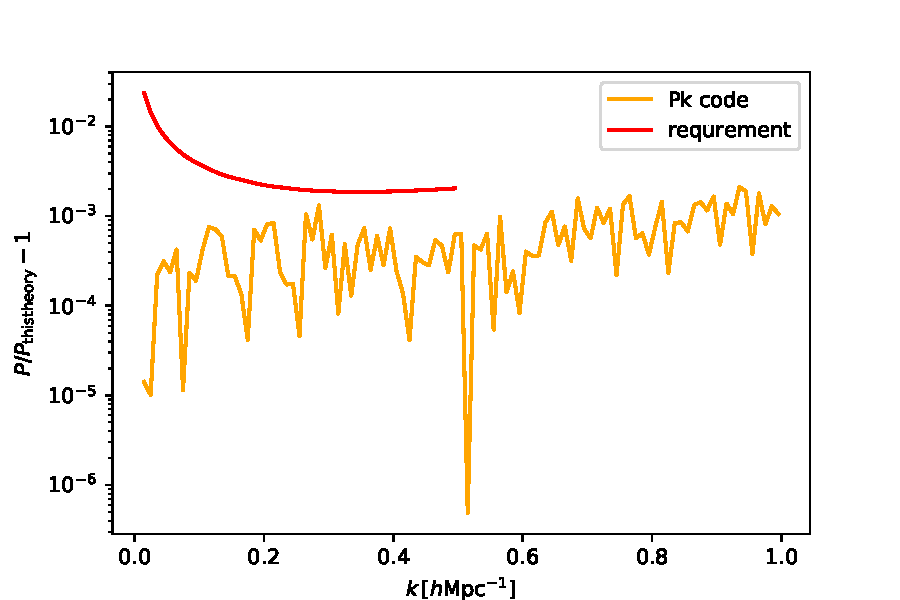
\includegraphics{zeldovich_linear3.pdf}
  \caption{Relative difference between the Zel'dovich power spectrum
    and the theoretical Zel'dovich power spectrum. The difference is
    below the science requirement.}
\end{figure}

\label{LastPage}
\end{document}

%
% 
%
